\documentclass[xcolor=dvipsnames]{beamer}
\usepackage{amsmath}
\usepackage{amssymb}
\usepackage[english]{babel}
\usepackage[latin1]{inputenc}
\usepackage{times}
\usepackage[T1]{fontenc}
\usepackage{graphicx}
\usepackage[absolute, overlay]{textpos}
\usepackage{tikz}
\usepackage{multimedia}
\usepackage{soul}
\usepackage{hyperref}
\usepackage{wasysym}
\usepackage{cancel}
\def\urltilda{\kern -.15em\lower .7ex\hbox{\~{}}\kern .04em}
\def\deg{^{\circ}}

\setlength{\TPHorizModule}{0.01\textwidth}
\setlength{\TPVertModule}{\TPHorizModule}

\definecolor{darkyellow}{rgb}{1,0.75,0}
\definecolor{black}{rgb}{0,0,0}
\definecolor{orange}{rgb}{0.9, 0.5, 0.0}

\mode<presentation>
{
  \usetheme{Warsaw}
  \usecolortheme[named=darkyellow]{structure}	
  \setbeamercovered{transparent}
  \setbeamercolor{item}{fg=black}
}

%\beamerdefaultoverlayspecification{<+->}

\newcommand{\vect}[1]{\boldsymbol{#1}}
\newcommand{\params}{\Xi}
\newcommand{\Eobsi}{E'_i}
\newcommand{\phiobsi}{\phi'_i}
\newcommand{\Etruei}{E_i}
\newcommand{\phitruei}{\phi_{i}}
\newcommand{\Eobsij}{E'_{ij}}
\newcommand{\phiobsij}{\phi'_{ij}}
\newcommand{\Etrueij}{E_{ij}}
\newcommand{\phitrueij}{\phi_{ij}}
\newcommand{\obs}{\mathrm{obs}}
\newcommand{\true}{\mathrm{true}}
\newcommand{\Like}{\mathcal{L}}
\newcommand{\ntot}{{n_\mathrm{tot}}}
\newcommand{\ntotj}{{n_{\mathrm{tot},j}}}
\newcommand{\diff}{\mathrm{d}}
\newcommand{\cblue}[1]{{\color[rgb]{0.1, 0.0, 0.6} #1}}
\newcommand{\cgreen}[1]{{\color[rgb]{0.0, 0.6, 0.1} #1}}
\newcommand{\corange}[1]{{\color[rgb]{0.9, 0.5, 0.0} #1}}
\newcommand{\cbluewhen}[2]{{\color#2[rgb]{0.1, 0.0, 0.6} #1}}
\newcommand{\cgreenwhen}[2]{{\color#2[rgb]{0.0, 0.6, 0.1} #1}}
\newcommand{\corangewhen}[2]{{\color#2[rgb]{0.9, 0.5, 0.0} #1}}
\newcommand{\vrel}{v_{\mathrm{rel}}}
\newcommand{\mn}{m_{\rm nuc}}
\newcommand{\mx}{m_\chi}
\newcommand{\nc}{\newcommand}
\nc{\x}{{\bf x }}
\nc{\kk}{{\bf k }}
\nc{\f}{{\bf f }}
\nc{\e}{{\bf e }}
\nc{\gag}{g_{a \gamma}}
\nc{\ud}{\mathrm{d}}
\nc{\igev}{GeV$^{-1}$}
\nc{\ssi}{\sigma_{\mathrm{SI}}}
\nc{\ssd}{\sigma_{\mathrm{SD}}}
\nc{\tq}{\tilde \q}
\nc{\qmin}{q_{\mathrm{min}}}
\nc{\qmax}{q_{\mathrm{max}}}
\nc{\dmin}{\delta_{\mathrm{min}}}
\nc{\dmax}{\delta_{\mathrm{max}}}
\nc{\ie}{i.e.\xspace}
\nc{\del}{\partial}
\nc{\Cin}{C_{\mathrm{in}}}
\nc{\Cout}{C_{\mathrm{out}}}
\nc{\shat}{\hat \sigma}
\nc{\ket}[1]{| #1 \rangle}
\nc{\bra}[1]{\langle #1 |}
\nc{\braket}[2]{\langle #1 | #2 \rangle}
\nc{\speclarrow}{$\boldsymbol{\rightarrow}$\ }
\nc{\bi}{\begin{itemize}}
\nc{\ei}{\end{itemize}}
\nc{\bfr}[1]{\begin{frame}\frametitle{#1}}

\AtBeginSection[]
{
  \begin{frame}<beamer>
    \frametitle{Outline}
  \begin{columns}[t]
	\column{0.8\textwidth}
	\tableofcontents[sections={1},currentsection,subsections]
        \vspace{3mm}
	\tableofcontents[sections={2},currentsection,subsections]
        \vspace{3mm}
	\tableofcontents[sections={3},currentsection,subsections]
  \end{columns}	
  \end{frame}
}

\setbeamertemplate{subsection in head/foot shaded}
{\textcolor{structure!80!black}{\insertsubsectionhead}}
\setbeamertemplate{subsection in head/foot}{\textcolor{black}\insertsubsectionhead}

\title[{\color[rgb]{0, 0, 0}Beyond the Standard Model with astro+particle physics}]{\textcolor{black}{Combining astrophysics with particle physics to get past the Standard Model}}
\author[Pat Scott -- April 11 -- RSAA]{Pat Scott}
\institute{\small{Imperial College London}}
\date[April 11, 2014]{Slides available from \color[rgb]{0.1, 0.0, 0.6} \href{http://www.physics.mcgill.ca/~patscott}{\tt www.physics.mcgill.ca/{\urltilda}patscott}}
\subject{Talks}

\begin{document}

\maketitle


\begin{frame}
  \frametitle{Outline}
  \begin{columns}[t]
	\column{0.8\textwidth}
	\tableofcontents[sections={1}]
        \vspace{3mm}
	\tableofcontents[sections={2}]
        \vspace{3mm}
	\tableofcontents[sections={3}]
  \end{columns}	
\end{frame}

\section{The Problem}

\begin{frame}
\frametitle{The Standard Model of particle physics}

\begin{columns}
\column{0.5\linewidth}
  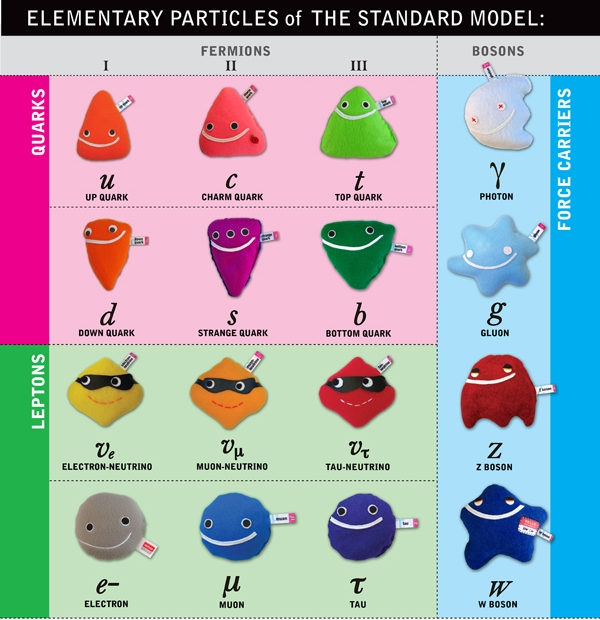
\includegraphics[width=\linewidth]{SM}
\column{0.12\linewidth}
  \centering
  \visible<2->{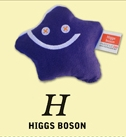
\includegraphics[width=\linewidth]{Higgs}}\vspace{5mm}
  \visible<4->{
\includegraphics[width=\linewidth]{DM}\\
  and friends$++$}
\end{columns}
\vspace{5mm}

\visible<3->{\cblue{19 free parameters}: (\alert{10} masses, \alert{3} force strengths, \alert{4} quark mixing parameters, \alert{2} `vacuumy things')}

\begin{textblock}{20}(82,35)
  \visible<5->{
    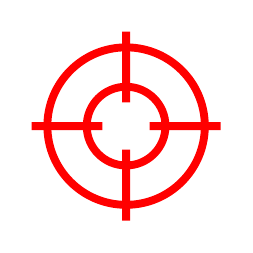
\begin{tikzpicture}
      \draw[color=red,line width=0.1cm]
            (0,0) circle (0.5)
            (0,0) circle (1) 
            (1.2,0) -- (0.3,0)
            (0,1.2) -- (0,0.3)
            (-1.2,0) -- (-0.3,0)
            (0,-1.2) -- (0,-0.3);
                   	
    \end{tikzpicture}
  }
\end{textblock}

\begin{textblock}{20}(84,58)
  \visible<6->{
    
\begin{tikzpicture}
      \draw[color=blue,line width=0.07cm]
            (0,0) circle (0.166)
            (0,0) circle (0.333) 
            (0.45,0) -- (0.1,0)
            (0,0.45) -- (0,0.1)
            (-0.45,0) -- (-0.1,0)
            (0,-0.45) -- (0,-0.1);
                   	
    \end{tikzpicture}
  }
\end{textblock}

\begin{textblock}{20}(90,60)
  \visible<7->{
    
\begin{tikzpicture}
      \draw[color=blue,line width=0.07cm]
            (0,0) circle (0.166)
            (0,0) circle (0.333) 
            (0.45,0) -- (0.1,0)
            (0,0.45) -- (0,0.1)
            (-0.45,0) -- (-0.1,0)
            (0,-0.45) -- (0,-0.1);
                   	
    \end{tikzpicture}
  }
\end{textblock}

\begin{textblock}{20}(95,57)
  \visible<8->{
    
\begin{tikzpicture}
      \draw[color=blue,line width=0.07cm]
            (0,0) circle (0.166)
            (0,0) circle (0.333) 
            (0.45,0) -- (0.1,0)
            (0,0.45) -- (0,0.1)
            (-0.45,0) -- (-0.1,0)
            (0,-0.45) -- (0,-0.1);
                   	
    \end{tikzpicture}
  }
\end{textblock}

\end{frame}

\begin{frame}
\frametitle{Searching for new physics}

\cblue{Many reasons to look for physics Beyond the Standard Model (BSM):}
\begin{itemize}
\item Higgs mass (hierarchy problem $+$ vacuum stability)
\item Dark matter exists
\item Baryon asymmetry
\item Neutrino masses and mixings
\end{itemize}

\visible<2->{
\cblue{So what do we do about it?}
\begin{itemize}
\item \cgreenwhen{Make new particles at high-$E$ colliders}{<3>}
\item \cgreenwhen{Study rare processes at high-$L$ colliders}{<3>}
\item \cgreenwhen{Hunt for dark matter (direct + indirect detection)}{<3>}
\item \cgreenwhen{Look at cosmological observables (CMB, reionisation, etc)}{<3>}
\item Look for kooky neutrino physics
\end{itemize}
}

\end{frame}

\begin{frame}
\frametitle{Combining searches {\rm I}}

  \begin{exampleblock}{Question}
  How do we know which models are in and which are out?
  \end{exampleblock} 

  \visible<2->{
  \begin{block}{Answer}
  Combine the results from different searches
  \end{block}

\begin{columns}[c]
\column{0.5\textwidth}
\footnotesize
\begin{itemize}
\item Simplest method: take different exclusions, overplot them, conclude things are ``allowed'' or ``excluded''
\item Simplest BSM example: the scalar singlet model
\vspace{1cm}
\end{itemize}
\column{0.45\textwidth}
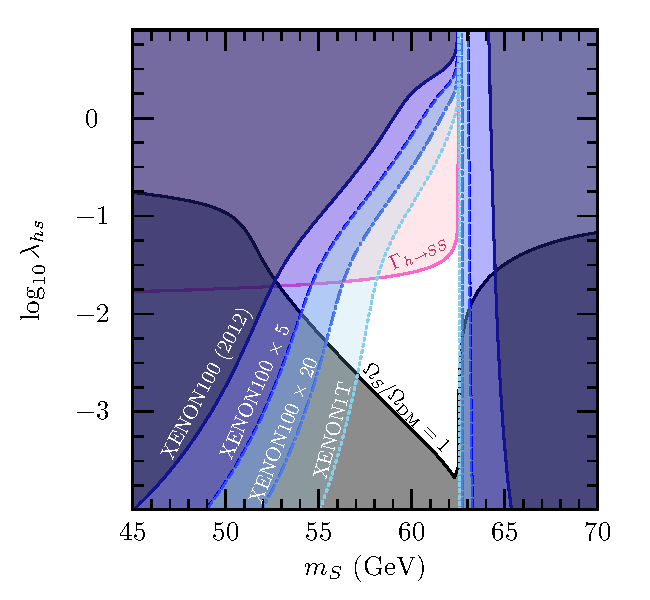
\includegraphics[width=\textwidth]{Fig6a}
\end{columns}
}

  \begin{textblock}{80}(20,75)
  \visible<2->{\tiny(Cline, Kainulainen, PS \& Weniger, \textit{PRD}, 1306.4710)}
  \end{textblock}

\end{frame}


\begin{frame}
\frametitle{Combining searches {\rm II}}

That's all well and good if there are only 2 parameters and few searches\ldots\vspace{3mm}

  \begin{exampleblock}{Question}
  What if there are many different \alert{constraints}?
  \end{exampleblock} 

  \visible<2->
  {
    \begin{columns}[c]
    \column{0.4\textwidth}
      \begin{block}{Answer}
        Combine constraints in a statistically valid way \\$\rightarrow$ composite likelihood
      \end{block}\vspace{10mm}
    \column{0.45\textwidth}
      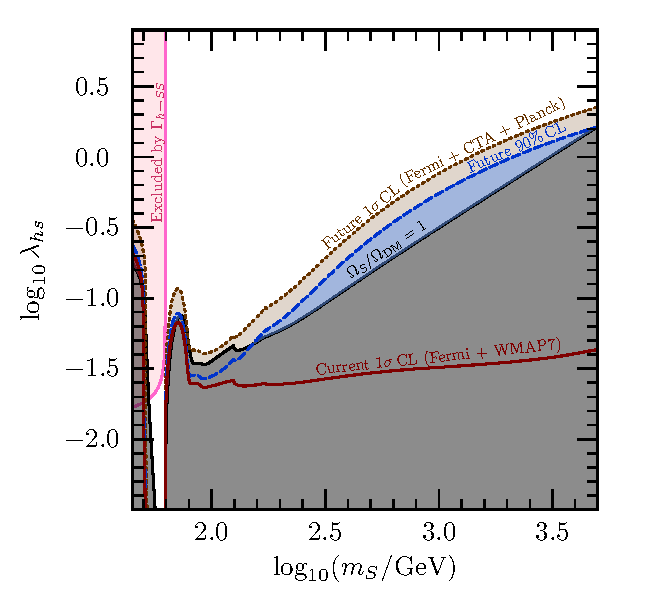
\includegraphics[width=\textwidth]{Fig3b}
    \end{columns}  
  }

  \begin{textblock}{80}(20,75)
  \visible<2->{\tiny(Cline, Kainulainen, PS \& Weniger, \textit{PRD}, 1306.4710)}
  \end{textblock}

\end{frame}


\begin{frame}
\frametitle{Combining searches {\rm III}}

That's all well and good if there are only 2 parameters and few searches\ldots\vspace{3mm}

  \begin{exampleblock}{Question}
  What if there are many \alert{parameters}?
  \end{exampleblock}

\visible<2->{
\begin{block}{Answer}
Need to 
\begin{itemize}
\item scan the parameter space (smart numerics)
\item interpret the combined results (Bayesian / frequentist)
\item project down to parameter planes of interest (marginalise / profile)
\end{itemize}
$\rightarrow$ \alert{global fits}
\end{block}}\vspace{3mm}

\end{frame}



\begin{frame}
\frametitle{Beyond-the-Standard-Model Scanning}

  \alert{Goals:} 
  \begin{enumerate} 
    \item Given a particular theory, determine which parameter combinations fit all experiments, and how well \visible<2->{\\\hspace{5.15cm}\cblue{$\implies$ parameter estimation}}
    \item Given multiple theories, determine which fit the data better, and quantify how much better \visible<2->{\cblue{$\implies$ model comparison}}
  \end{enumerate} 
  \vspace{4mm}

\visible<3>{
Why simple IN/OUT analyses are not enough\ldots
\vspace{2mm}

\begin{itemize}
\item Only partial goodness of fit, no measure of convergence, no idea how to generalise to regions or whole space.
\item Frequency/density of models in IN/OUT scans is \\\alert{not} proportional to probability $\implies$ means essentially \alert{nothing}.
\item Sadly, some people still do this\ldots
\end{itemize}
\vspace{3mm}

}

\end{frame}

\begin{frame}
\frametitle{Know your (supersymmetric) parameter scans}

\begin{columns}[c]
\column{0.3\linewidth}
\textbf{Global fits:}\\
\footnotesize\vspace{2mm}
Quantitative?\\
\hspace{2mm}per-point: always\\
\hspace{2mm}overall: always\vspace{15mm}

\textbf{Not global fits:}\\
\footnotesize\vspace{2mm}
Quantitative?\\
\hspace{2mm}per-point: sometimes\\
\hspace{2mm}overall: never\vspace{5mm}


\column{0.35\linewidth}
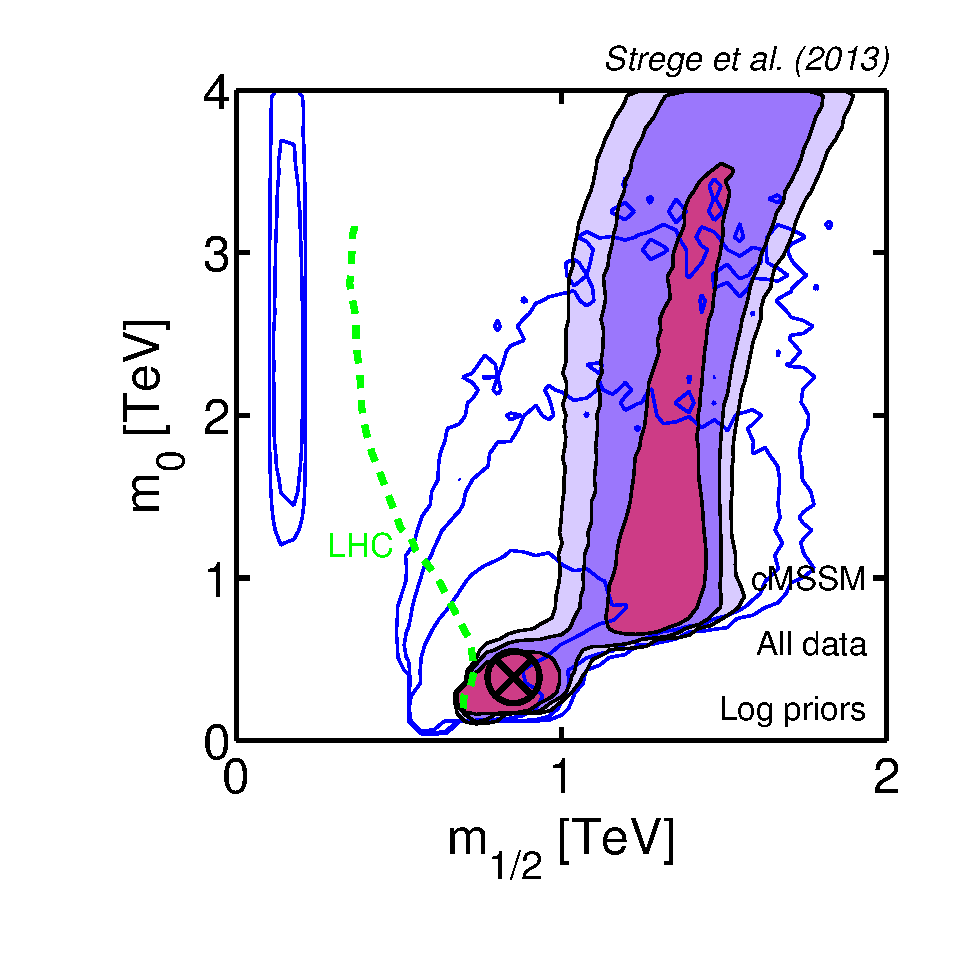
\includegraphics[width=0.8\textwidth, trim = 40 40 0 40, clip=true]{Strege13}\\\vspace{-1mm}
{\tiny Strege et al \textit{JCAP}, 1212.2636}\\\vspace{3mm}
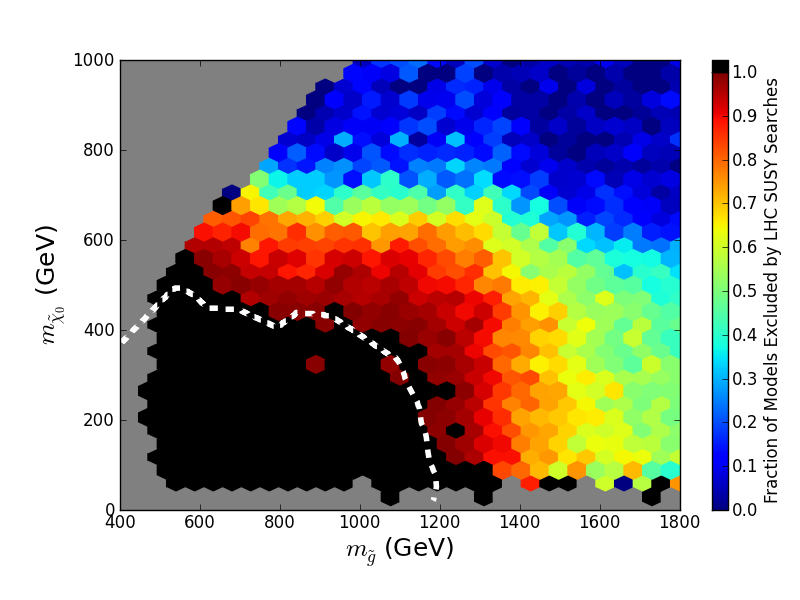
\includegraphics[width=\textwidth]{LSP_Gluino_13_Efficiency}\\
{\tiny Cahill-Rowley et al, 1307.8444}\\\vspace{3mm}

\column{0.35\linewidth}
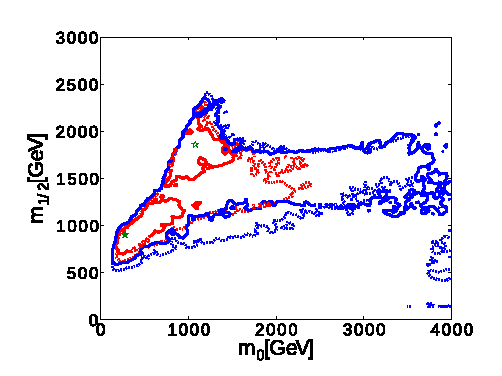
\includegraphics[width=\textwidth]{MasterCode2012_CMSSM}\\\vspace{-1mm}
{\tiny MasterCode, \textit{EPJC}, 1207.7315}\vspace{3mm}
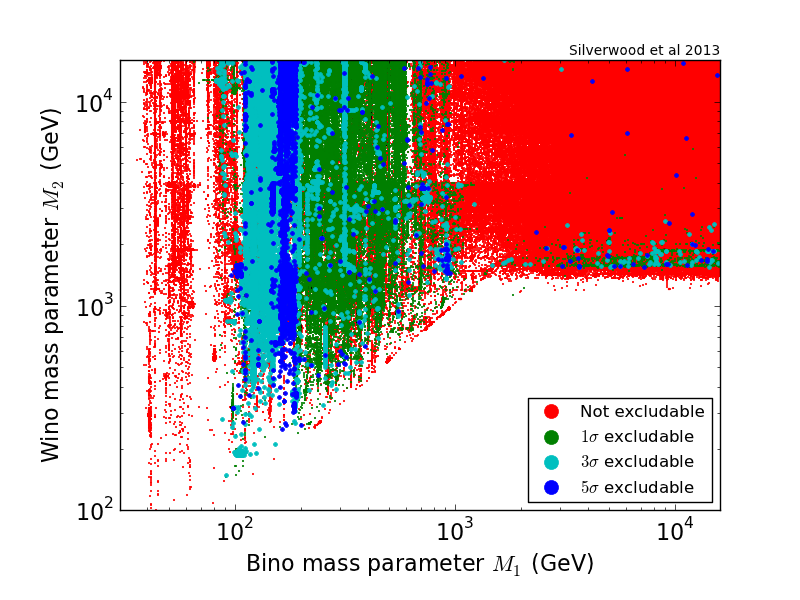
\includegraphics[width=\textwidth]{PvP1_Outm1_v_Outm2}\\
{\tiny Silverwood, PS, et al, \textit{JCAP}, 1210.0844}\vspace{3mm}

\end{columns}

\end{frame}

\begin{frame}
\frametitle{Putting it all together}  

  \alert{Issue 1:} Combining fits to different experiments\\
  Relatively easy -- composite likelihood ($\mathcal{L}_1\times\mathcal{L}_2 \equiv \chi^2_1 + \chi^2_2$ for simplest $\mathcal{L}$)
  {\footnotesize\begin{itemize}
    \item{dark matter relic density from WMAP/Planck}
    \item{precision electroweak tests at LEP}
    \item{LEP limits on new particle particle masses}
    \item{$B$-factory data (rare decays, $b\rightarrow s\gamma$)}
    \item{muon anomalous magnetic moment}
    \item{LHC searches, direct detection}
  \end{itemize}}
  \vspace{2mm}

\end{frame}

\begin{frame}
\frametitle{Putting it all together: global fits}  

  \alert{Issue 2:} Including the effects of uncertainties in input data\\
  Easy -- treat them as \emph{nuisance parameters} and profile/marginalise\vspace{4mm}

  \alert{Issue 3:} Finding the points with the best likelihoods\\
  Tough -- MCMCs, nested sampling, genetic algorithms, etc\vspace{4mm}

  \alert{Issue 4:} Comparing theories\\
  Depends -- Bayesian model comparison, $p$ values\\
  \hspace{40mm}($TS$ distribution? $\longrightarrow$ coverage???) 

\end{frame}

\begin{frame}
\frametitle{Progress including searches for dark matter}

  \begin{itemize}
  \item
  \visible<2->{Direct detection -- nuclear collisions and recoils \\(\cgreen{yes: XENON100 approximate likelihoods})\vspace{1mm}}
  \item
  \visible<3->{Direct production -- missing $E_\mathrm{T}$ or otherwise -- LHC, Tevatron (\alert{not really yet})\vspace{1mm}}
  \item
  \visible<4->{Indirect detection -- annihilations producing
  \begin{itemize}
    \footnotesize
    \visible<5->{\item{gamma-rays -- \emph{Fermi}, HESS, CTA (\cgreen{yes: Fermi, HESS dwarfs})}\vspace{1mm}}
    \visible<6->{\item{anti-protons -- PAMELA, AMS (\alert{not yet})}\vspace{1mm}}
    \visible<7->{\item{anti-deuterons -- GAPS (\alert{not yet}) }\vspace{1mm}}
    \visible<8->{\item{neutrinos -- IceCube, ANTARES (\cgreen{yes: IceCube 22-string})}\vspace{1mm}}
    \visible<9->{\item{$e^+e^-$ -- PAMELA, \emph{Fermi}, ATIC, AMS (\alert{not yet})}\vspace{1mm}}
    \visible<10->{\item{secondary impacts on the CMB (\cgreen{yes: WMAP5})}\vspace{1mm}}
  \end{itemize}}
  \end{itemize}

\begin{textblock}{70}(84,51)
\visible<5->
{
  \tiny
  PS, Conrad et al {\it JCAP}, 0909.3300\\
  Ripken, Conrad \& PS {\it JCAP}, 1012.3939\\
}
\end{textblock}

\begin{textblock}{35}(84,65)
\visible<8->
{
  \tiny
  PS, Savage,  Edsj\"o \& The IceCube Collab. {\it JCAP}, 1207.0810\\ 
  Silverwood, PS et al \textit{JCAP}, 1210.0844\\
}
\end{textblock}

\begin{textblock}{70}(84,29)
\visible<2->
{
  \tiny
  Strege et al \textit{JCAP}, 1212.2636\\
}
\end{textblock}

\begin{textblock}{70}(84,73)
\visible<10->
{
  \tiny
  Cline \& PS \textit{JCAP}, 1301.5908
}
\end{textblock}

\end{frame}


\begin{frame}
\frametitle{Example of Combined Direct + Indirect + LHC constraints}

\Large

\visible<1-4>{Base Observables} \visible<2-4>{$+$ XENON-100}\only<2>{ (2011)} \only<3-4>{$+$ CMS\,5\,fb$^{-1}$}

{\centering \visible<4>{$+$ projected IC86-DeepCore}}

\vspace{2mm}
\footnotesize
\visible<2-4>{Grey contours correspond to Base Observables \textit{only}}
\vspace{2mm}

\begin{columns}
\column{0.36\textwidth}
\only<1>{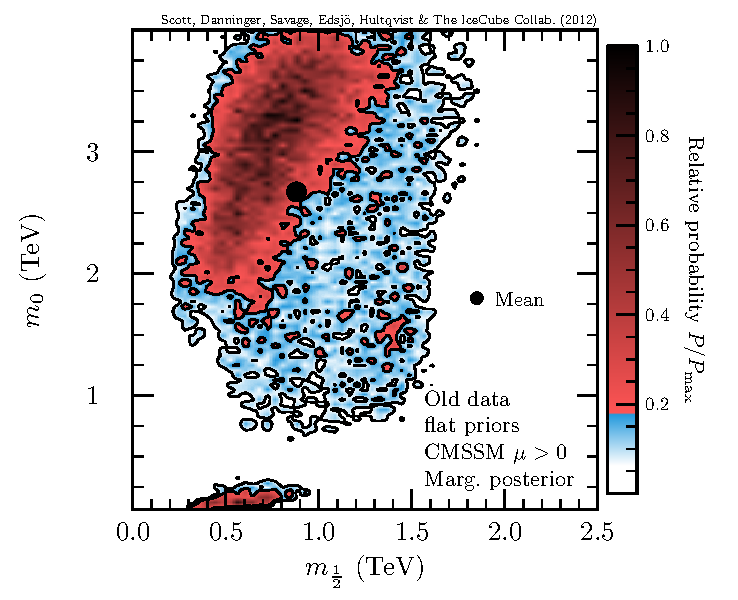
\includegraphics[height=0.92\linewidth, trim = 8 0 30 0, clip = true]{marg2D_1_1}}%
\only<2>{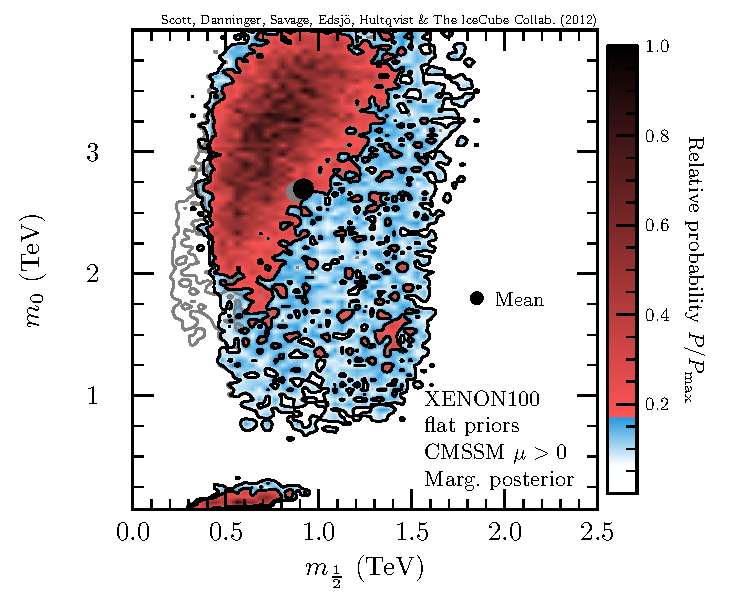
\includegraphics[height=0.92\linewidth, trim = 8 0 30 0, clip = true]{marg2D_2_1}}%
\only<3>{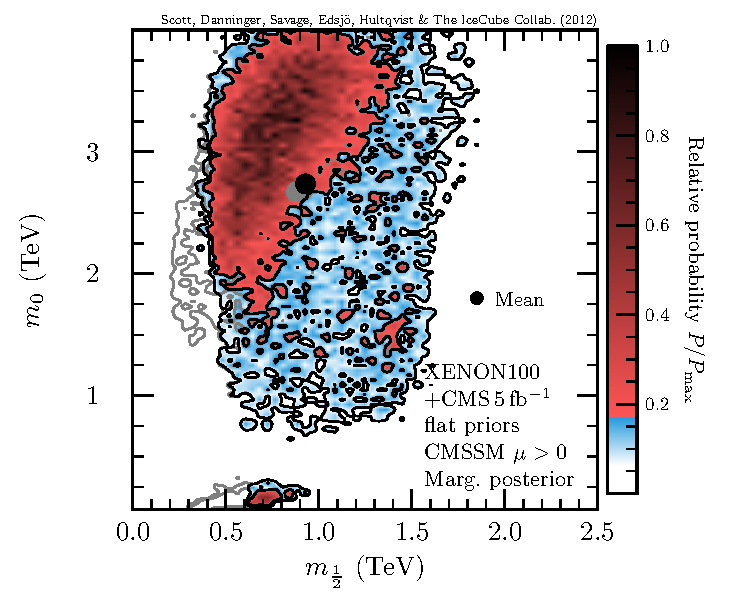
\includegraphics[height=0.92\linewidth, trim = 8 0 30 0, clip = true]{marg2D_3_1}}%
\only<4>{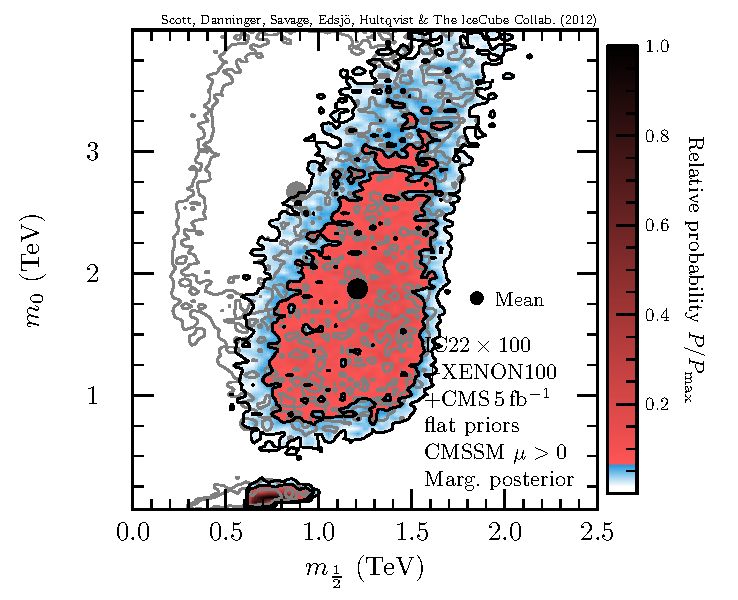
\includegraphics[height=0.92\linewidth, trim = 8 0 30 0, clip = true]{marg2D_4_1}}
\column{0.36\textwidth}
\only<1>{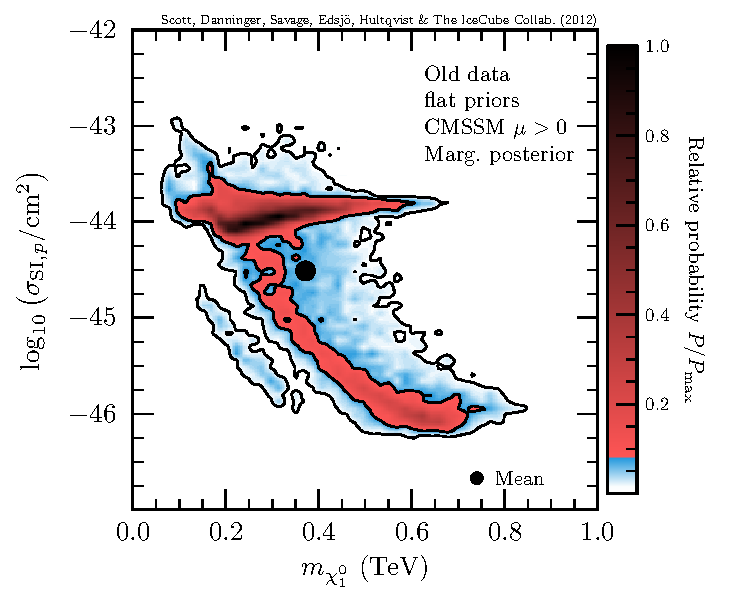
\includegraphics[height=0.92\linewidth, trim = 8 0 30 0, clip = true]{marg2D_1_2}}%
\only<2>{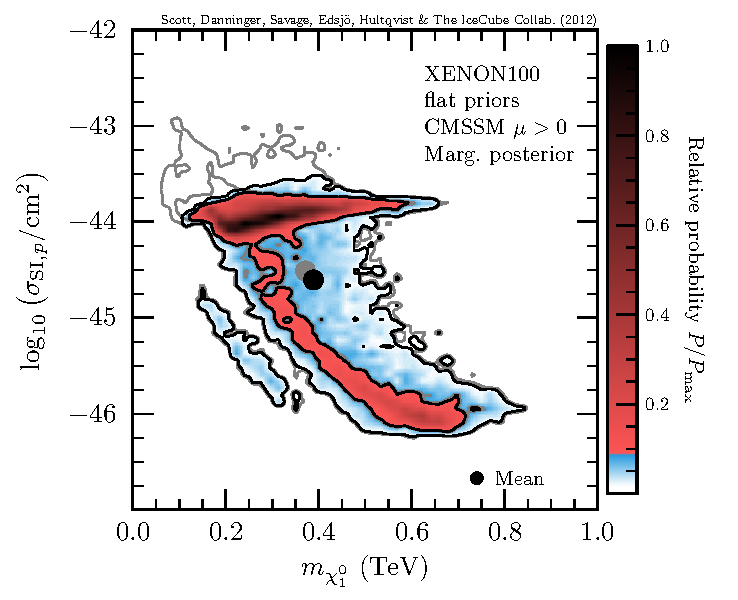
\includegraphics[height=0.92\linewidth, trim = 8 0 30 0, clip = true]{marg2D_2_2}}%
\only<3>{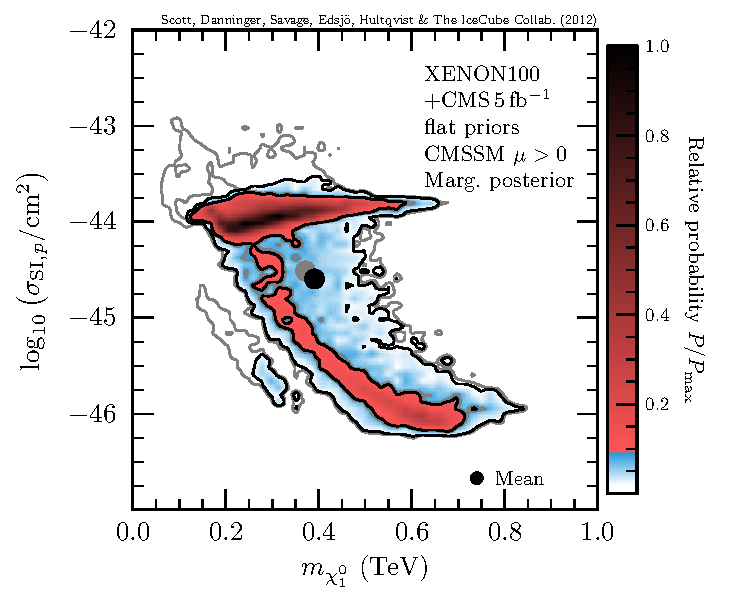
\includegraphics[height=0.92\linewidth, trim = 8 0 30 0, clip = true]{marg2D_3_2}}%
\only<4>{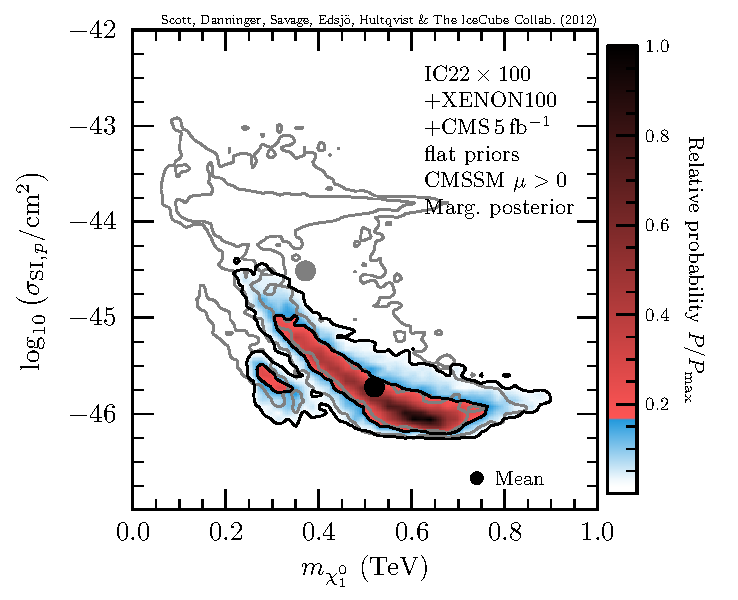
\includegraphics[height=0.92\linewidth, trim = 8 0 30 0, clip = true]{marg2D_4_2}}
\column{0.36\textwidth}
\only<1>{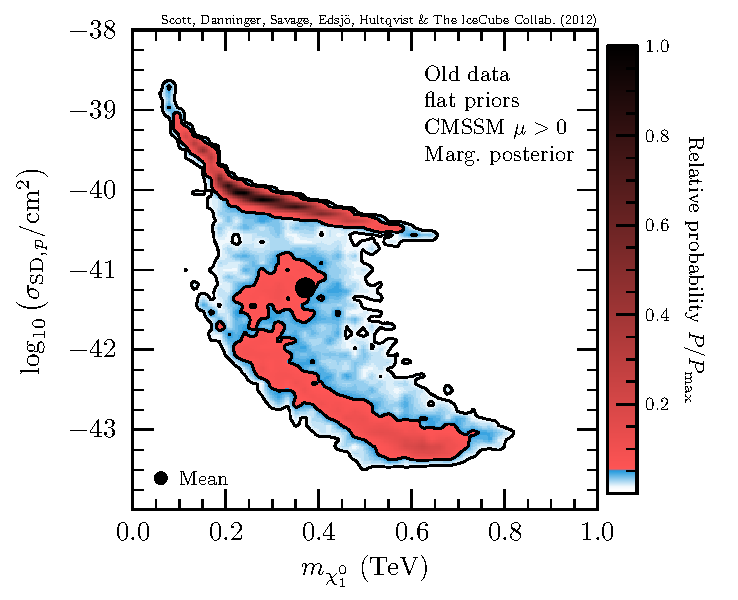
\includegraphics[height=0.92\linewidth, trim = 8 0 10 0, clip = true]{marg2D_1_3}}%
\only<2>{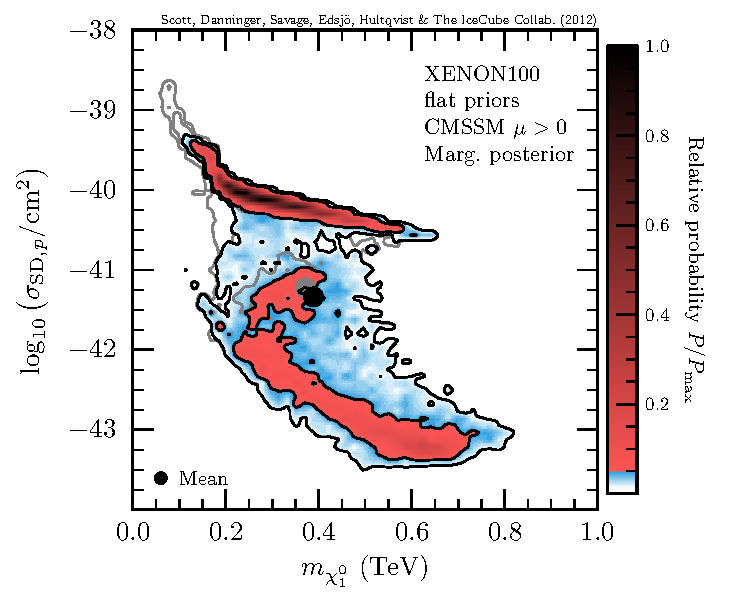
\includegraphics[height=0.92\linewidth, trim = 8 0 10 0, clip = true]{marg2D_2_3}}%
\only<3>{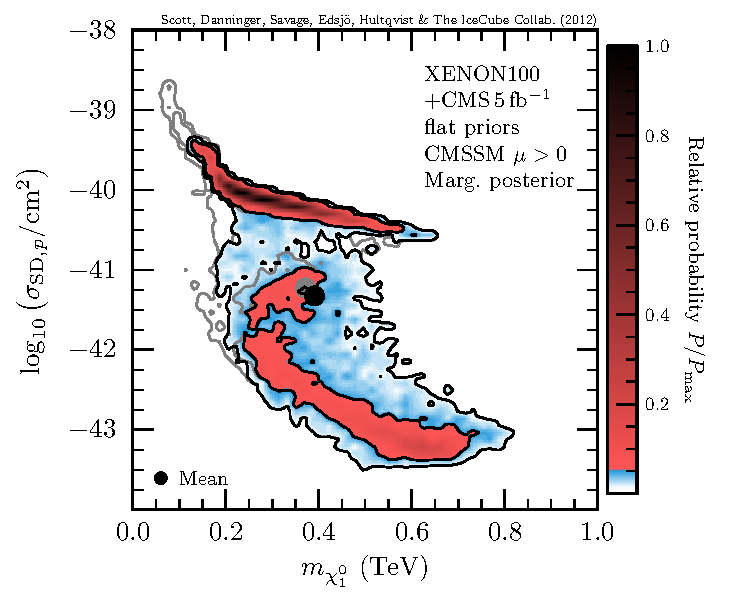
\includegraphics[height=0.92\linewidth, trim = 8 0 10 0, clip = true]{marg2D_3_3}}%
\only<4>{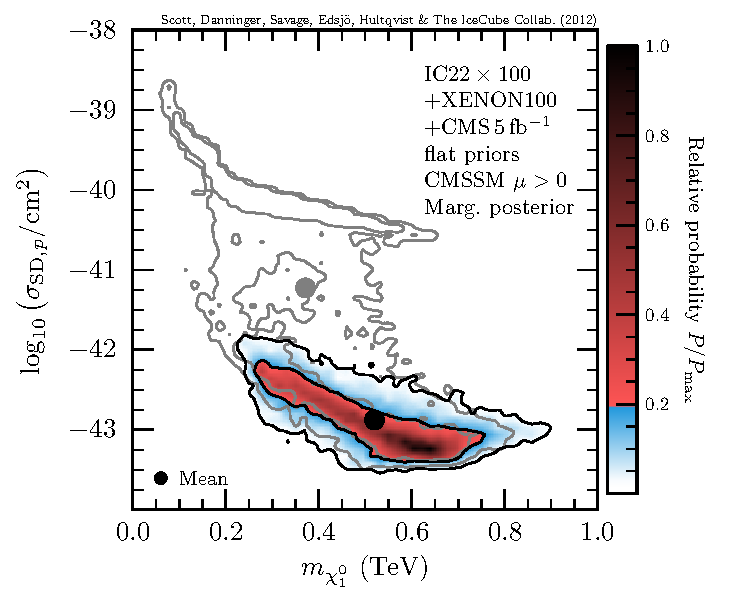
\includegraphics[height=0.92\linewidth, trim = 8 0 10 0, clip = true]{marg2D_4_3}}
\end{columns}
\vspace{2mm}

\visible<4>{\textbf{CMSSM, IceCube-22 with 100$\times$ boosted effective area}\\
(kinda like IceCube-DeepCore)}

\end{frame}


\section{Future Challenges}

\subsection{Respectable LHC likelihoods}

\begin{frame}
\frametitle{The LHC likelihood monster}

\begin{textblock}{30}(80.6,10.2)
    
\includegraphics[width=\linewidth]{LHCmonster}
\end{textblock}

\visible<1->{
\begin{exampleblock}{Time per point:}
$\mathcal{O}(minute)$ in \alert{best} cases
\end{exampleblock}
}

\visible<2->{
\begin{exampleblock}{Time per point for global fits to converge:}
$\mathcal{O}(seconds)$ in \alert{worst} cases
\end{exampleblock}
}

\visible<3->{
\begin{exampleblock}{Challenge:}
About 2 orders of magnitude too slow to actually include LHC data in global fits properly
\end{exampleblock}
}

\end{frame}

\begin{frame}
\frametitle{Taming the LHC monster}

\only<1,2>{
\begin{exampleblock}{Zeroth Order Response:}
``Stuff it, just use the published limits and ignore the dependence on other parameters''
\end{exampleblock}

\visible<2>{
\vspace{5mm}
Obviously naughty -- plotted limits assume CMSSM, and fix two of the parameters
\begin{itemize}    
  \item Don't really know dependence on other parameters
  \item Don't have a likelihood function, just a line
  \item Can't use this at all for non-CMSSM global fits -- e.g. MSSM-25
\end{itemize}

\vspace{5mm}
SuperBayeS
}}  

\only<3,4>{
\begin{exampleblock}{First Order Response:}
``Test if things depend on the other parameters (hope not), re-simulate published exclusion curve''
\end{exampleblock}

\visible<4>{
\vspace{5mm}
Not that great, but OK in some cases
\begin{itemize}    
  \item At least have some sort of likelihood this time
  \item Still a bit screwed if things do depend a lot on other parameters, but
  \item allows (potentially shaky) extrapolation, also to non-CMSSM models
\end{itemize}

\vspace{5mm}
Fittino, Mastercode
}}

\only<5,6>{
\begin{exampleblock}{Second Order Response:}
``That's ridiculous.  I've never met a calculation I can't speed up.  There must be some way to have my cake and eat it too''
\end{exampleblock}

\visible<6>{
\vspace{5mm}
Maybe -- this is the challenge.
\begin{itemize}    
  \item Interpolated likelihoods (how to choose nodes?)
  \item Neural network functional approximation (how to train accurately?)
  \item Some sort of smart reduction based on event topology? 
  \item Something else?
\end{itemize}

\vspace{5mm}
Bal\'azs, Buckley, Farmer, White et al (1106.4613, 1205.1568); GAMBIT  
}}

\end{frame}


\subsection{Parameter space $\rightarrow$ Theory space}

\begin{frame}
\frametitle{CMSSM, SMS $\ne$ BSM}

(SMS = Simplified Model Spectrum)
\vspace{3mm}

Want to do model comparison to actually work out which theory is right\ldots
\vspace{3mm}

\begin{exampleblock}{Challenge:}
How do I easily adapt a global fit to different BSM theories?
\end{exampleblock}

\visible<2>{
Somehow, we must recast things quickly to a new theory 
\begin{itemize}
\item data
\item likelihood functions
\item scanning code `housekeeping'
\item even predictions
\end{itemize}
$\implies$ a new, very abstract global fitting framework
}

\end{frame}

\begin{frame}
\frametitle{Hitting the wall}

Issues with current global fit codes:
\begin{itemize}
\item Strongly wedded to a few theories (e.g. constrained MSSM / mSUGRA)
\item Strongly wedded to a few theory calculators
\item All datasets and observables basically hardcoded
\item Rough or non-existent treatment of most experiments (astroparticle + collider especially)
\item Sub-optimal statistical methods / search algorithms
\item $\implies$ \textit{already hitting the wall on theories, data \& computational methods}
\end{itemize}

\end{frame}

\begin{frame}
\frametitle{\textbf{GAMBIT}: a \textit{second-generation} global fit code}

GAMBIT: \alert{G}lobal \alert{A}nd \alert{M}odular \alert{B}SM \alert{I}nference \alert{T}ool
\vspace{5mm}

Overriding principles of GAMBIT: flexibility and modularity
\begin{itemize}
\item General enough to allow fast definition of new datasets and theoretical models
\item Plug and play scanning, physics and likelihood packages
\item Extensive model database -- not just small modifications to constrained MSSM (NUHM, etc), and not just SUSY!
\item Extensive observable/data libraries (likelihood modules)
\item Many statistical options -- Bayesian/frequentist, likelihood definitions, scanning algorithms
\item A smart and \textit{fast} LHC likelihood calculator
\item Massively parallel
\item Full open-source code release
\end{itemize}

\end{frame}


\begin{frame}
\frametitle{The GAMBIT Collaboration}

\vspace{6mm}
23 Members, 13 Institutes \\
8 Experiments, 4 major theory codes \vspace{3mm}

\begin{tabular}{l l}
\textbf{Fermi-LAT} & \small J.\ Conrad, J.\ Edsj\"o, G.\ Martinez, \cgreenwhen{P.\ Scott}{<2>} (leader)\\
\textbf{CTA} & \small C. Bal\'azs, T.\ Bringmann, J.\ Conrad, \cgreenwhen{M.\ White}{<2>} (dep.\ leader)\\
\textbf{ATLAS} & \small A.\ Buckley, \cgreenwhen{P.\ Jackson}{<2>}, C.\ Rogan, \cgreenwhen{A.\ Saavedra}{<2>}, \cgreenwhen{M.\ White}{<2>}\\
\textbf{IceCube} & \small J.\ Edsj\"o, C.\ Savage, \cgreenwhen{P.\ Scott}{<2>}\\
\textbf{LHCb} & \small N.\ Serra\\
\textbf{HESS} & \small J.\ Conrad \\
\textbf{AMS-02} & \small A.\ Putze\\
\textbf{DARWIN} & \small J.\ Conrad\\
\textbf{Theory} & \small \cgreenwhen{P.\ Athron, C. Bal\'azs}{<2>}, T.\ Bringmann, J.\ Cornell, L.-A.\ Dal, \\
                & \small J.\ Edsj\"o, \cgreenwhen{B.\ Farmer}{<2>}, A.\ Krislock, A.\ Kvellestad, \\
                & \small N.\ Mahmoudi, A.\ Raklev, C.\ Savage, \cgreenwhen{P.\ Scott}{<2>}, C.\ Weniger, \\
                & \cgreenwhen{M.\ White}{<2>} \\	
\end{tabular}

\begin{textblock}{25}(95,10)
  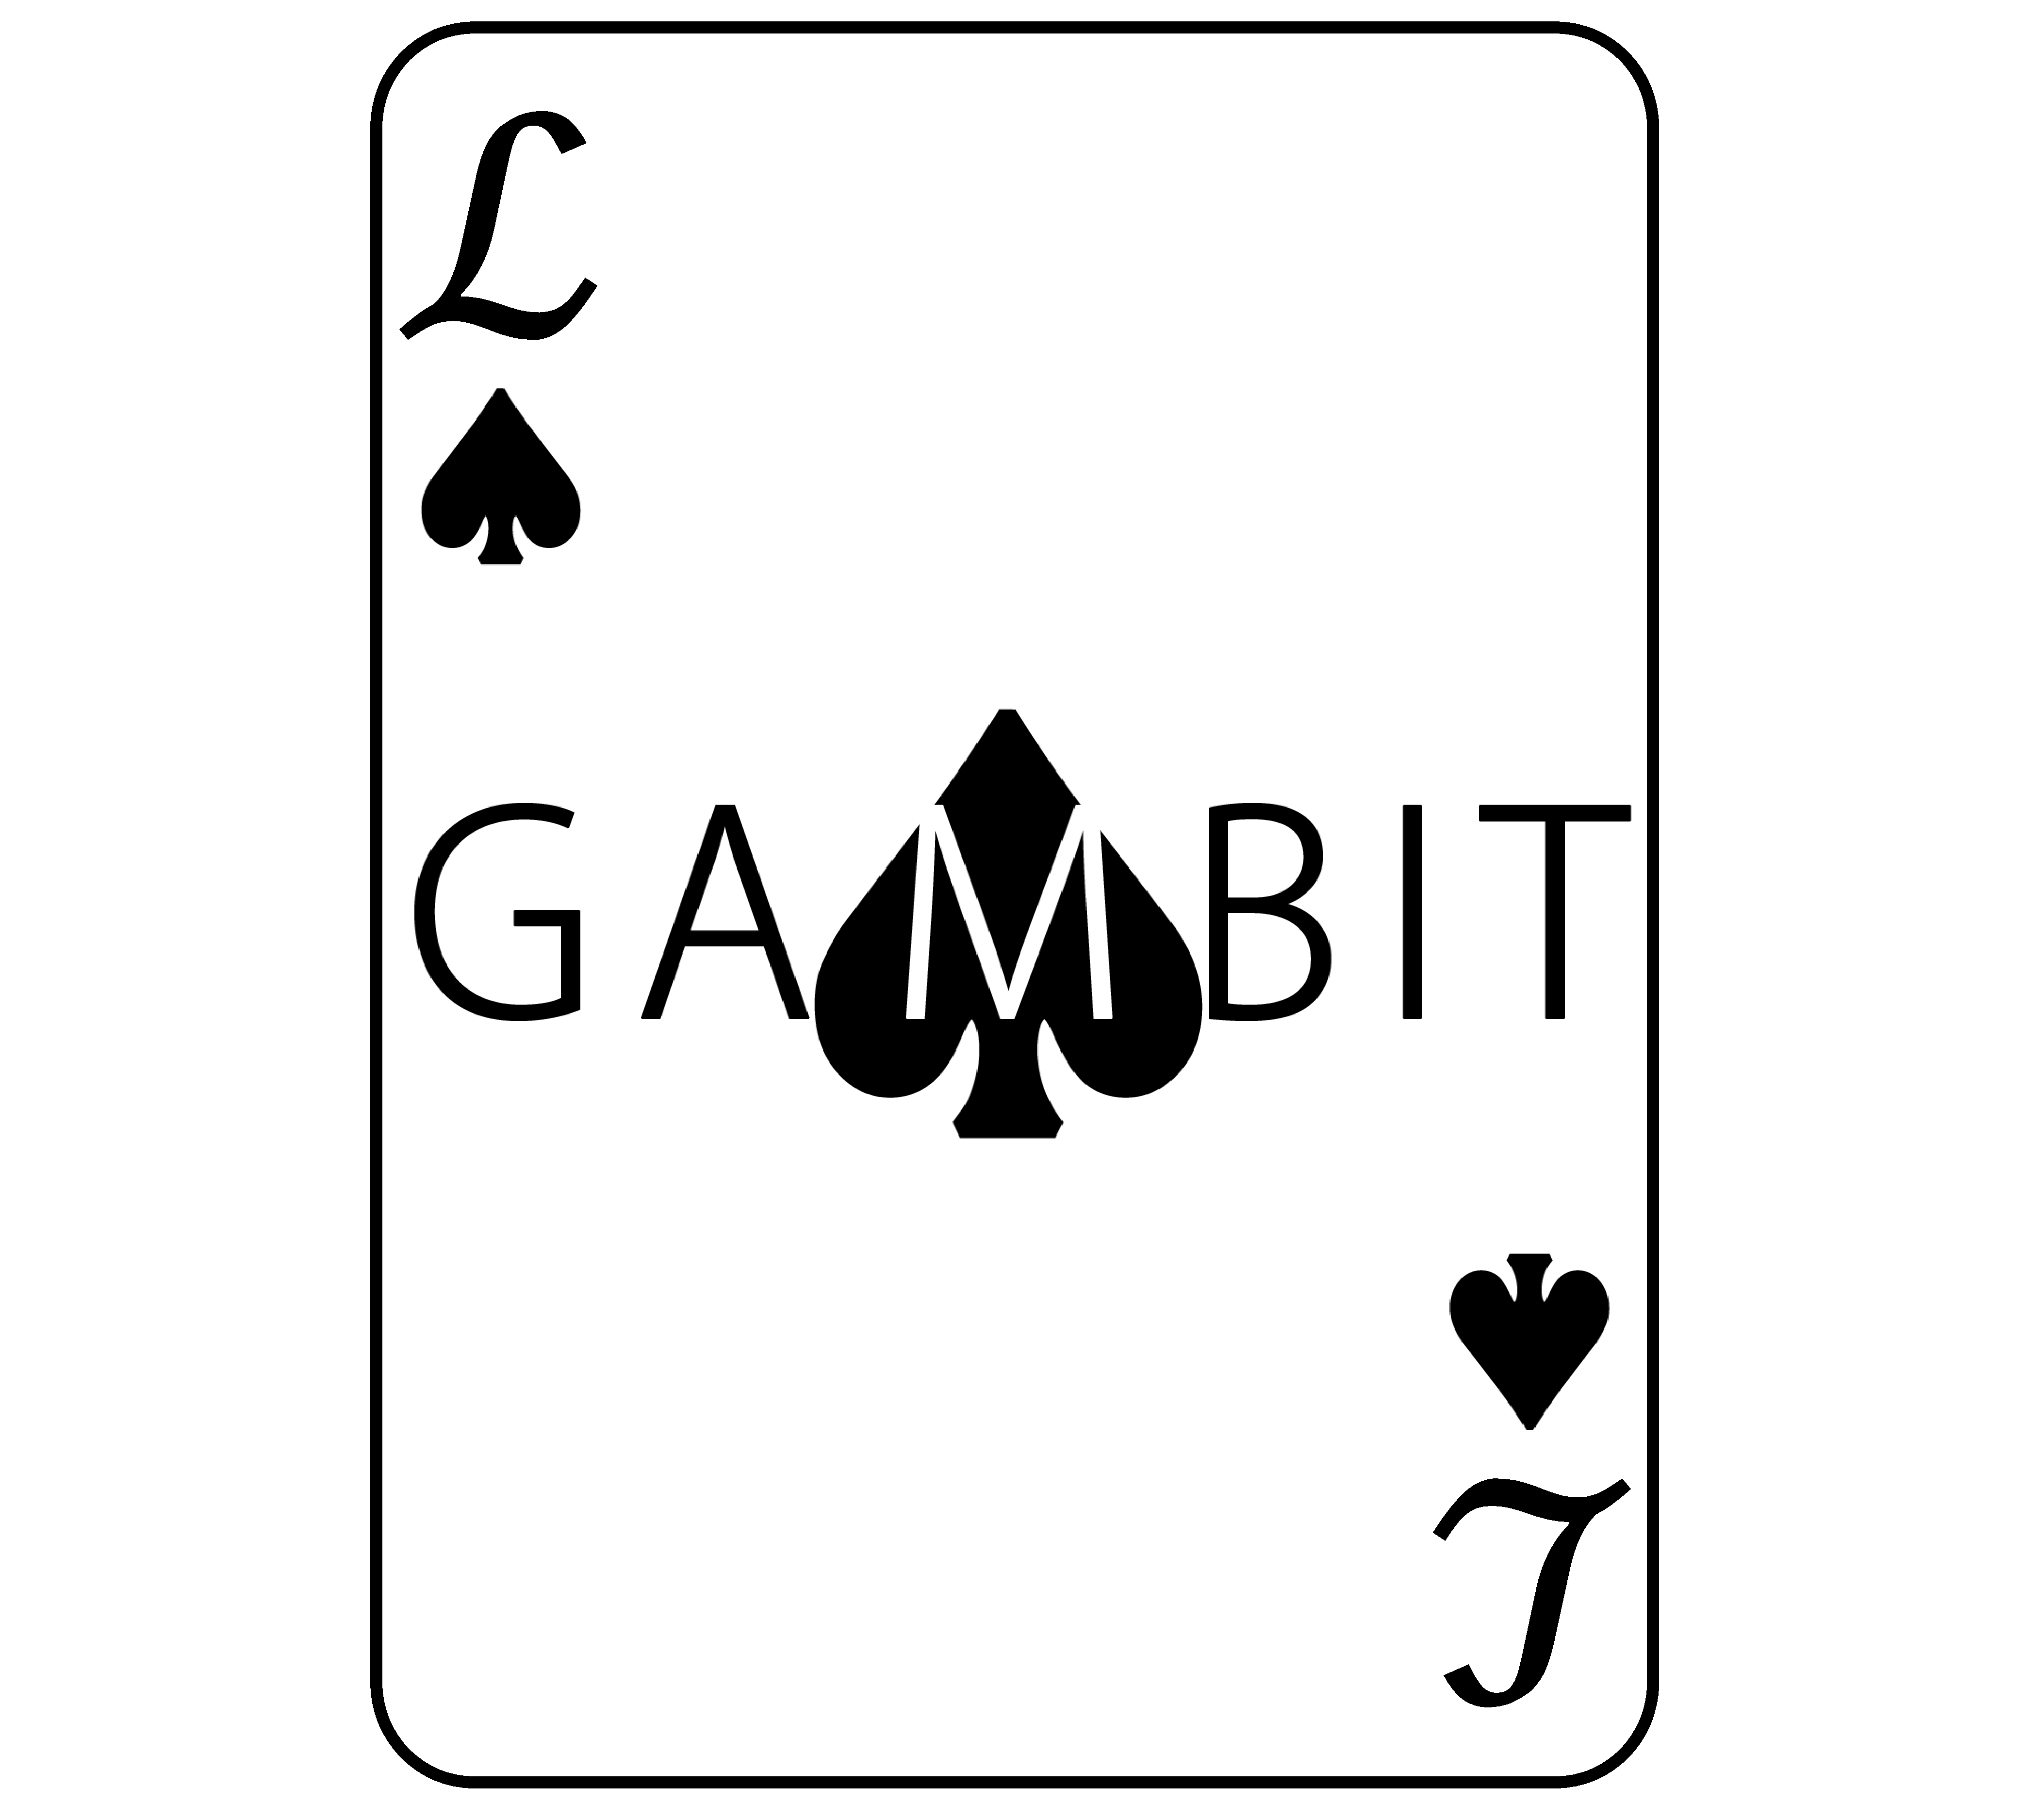
\includegraphics[width=\linewidth]{Logo_Final}	
\end{textblock}


\end{frame}

\begin{frame}
\frametitle{Closing remarks}

\begin{itemize}
\item{Robust analysis of dark matter and BSM physics requires multi-messenger global fits}
\item{GAMBIT is coming:}\bi
\item[$\rightarrow$]{\alert{Lots} of interesting particle, astronomical, cosmological and astroparticle observables to include in global fits}
\item[$\rightarrow$]{Serious theoretical, experimental, statistical and computational detail to work though}
\item[$\rightarrow$]{\alert{Many} opportunities for good students}\ei
\end{itemize}


\end{frame}

\appendix

\section{Backup Slides}

\begin{frame}
\frametitle{GAMBIT: sneak peek}
\centering
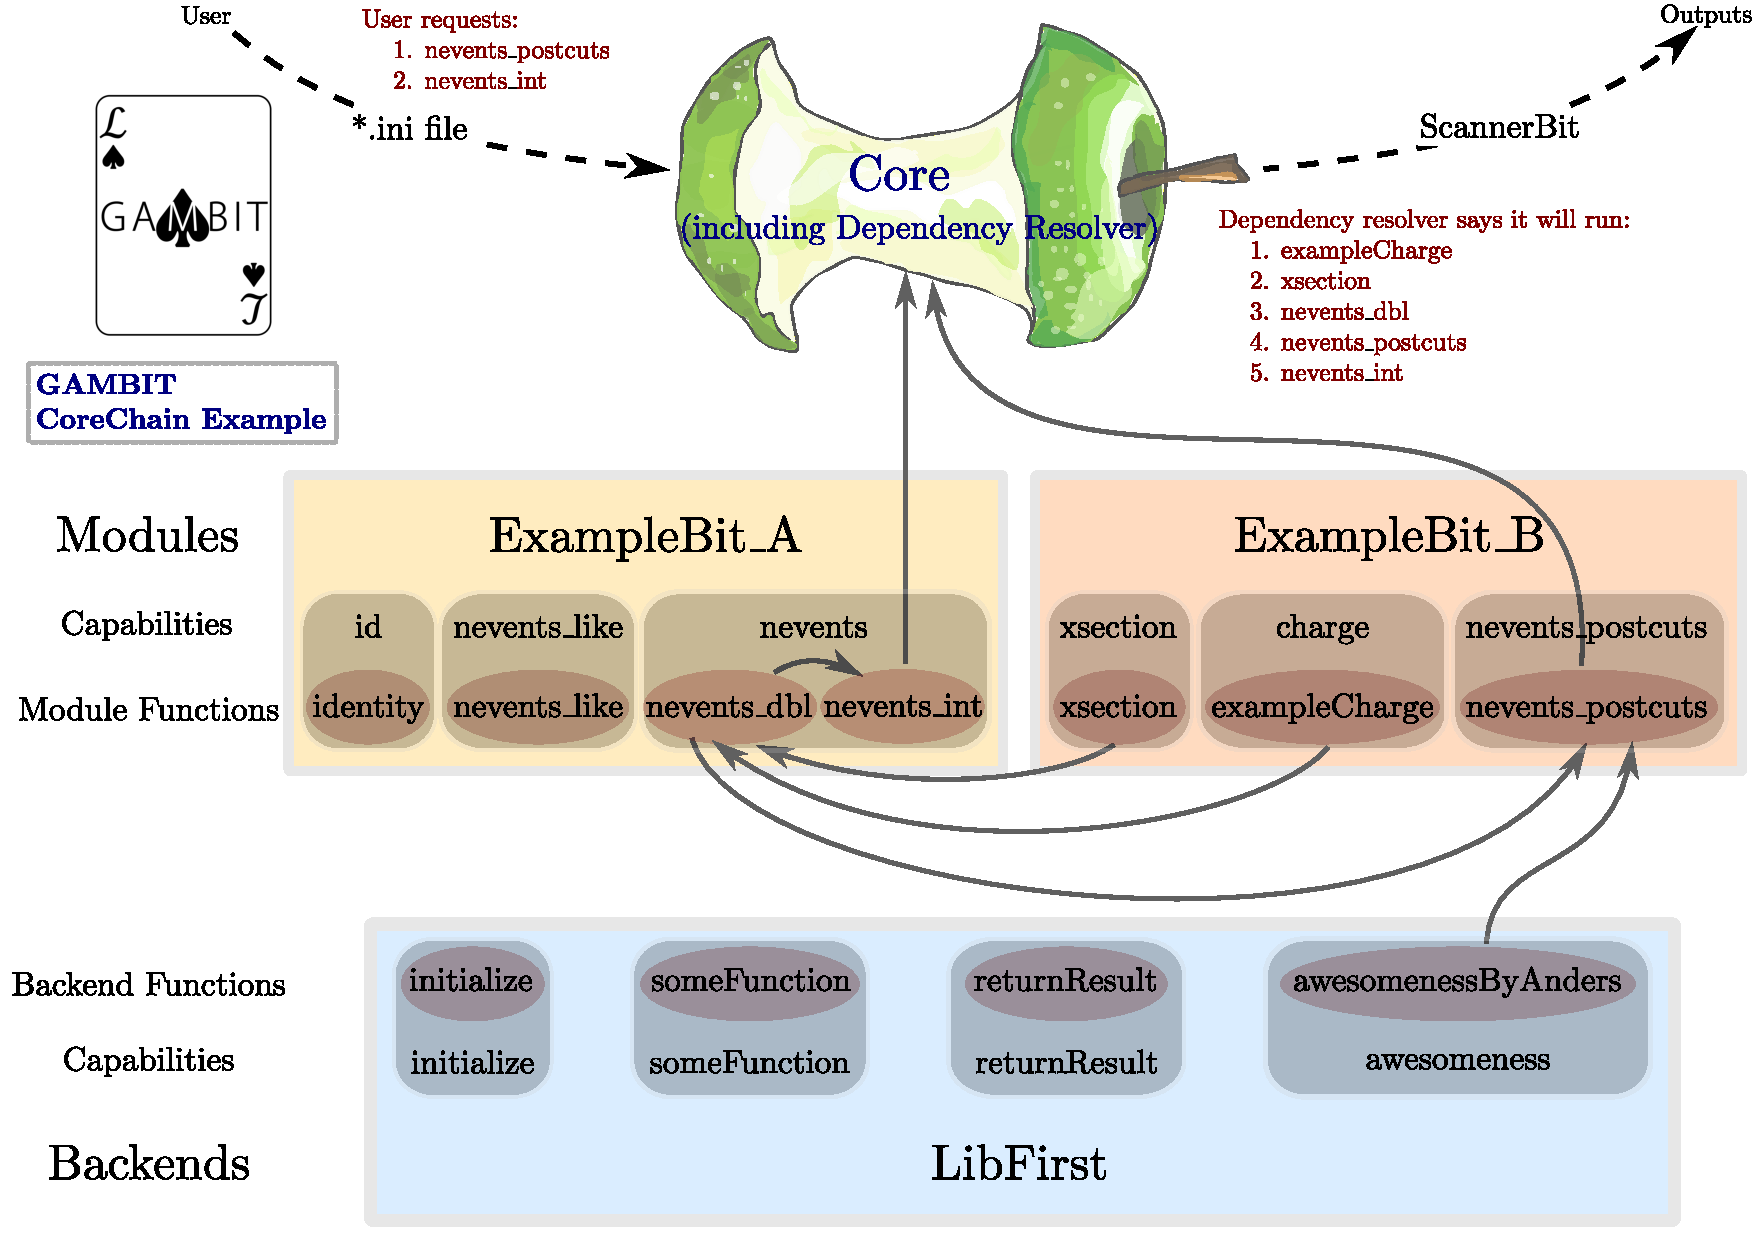
\includegraphics[width=0.9\textwidth]{coreChainDiagram_example_wlogo}	
\end{frame}

\begin{frame}
\frametitle{Scanning algorithms}

\cblue{Convergence remains an issue, especially for profile likelihood}\\
Messy likelihood $\implies$ best-fit point can be (and often is) easily missed {\tiny(Akrami, PS et al {\it JHEP}, 0910.3950, Feroz et al {\it JHEP}, 1101.3296)}
      \begin{itemize}\footnotesize
                 \item frequentist CLs are off, as isolikelihood levels are chosen incorrectly
                 \item can impact coverage (overcoverage, or masking of undercoverage due to non-$\chi^2$ $TS$ distribution)
                 \item need to use multiple priors and scanning algorithms (one optimised for profile likelihoods?)  
      \end{itemize}\vspace{-2mm}
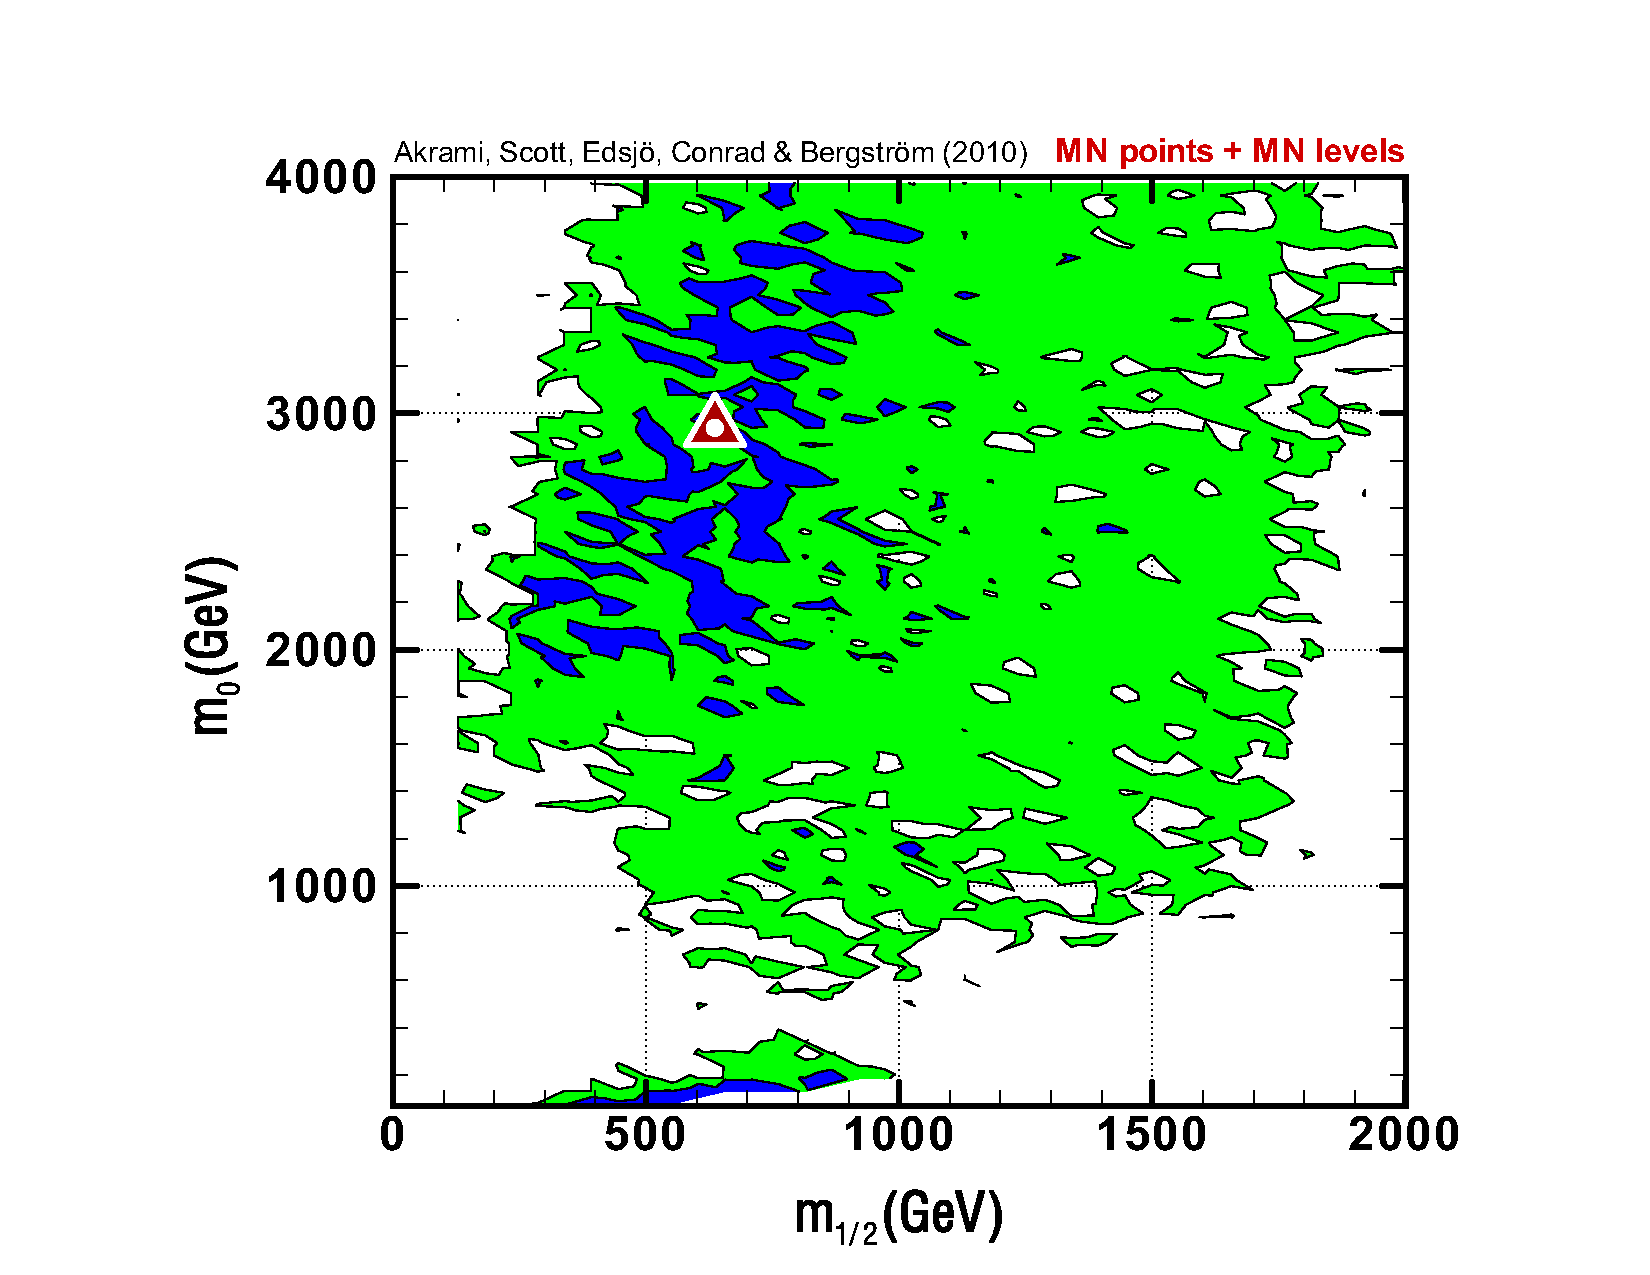
\includegraphics[width=0.5\textwidth]{MN_m0mhf_MNlevels}	
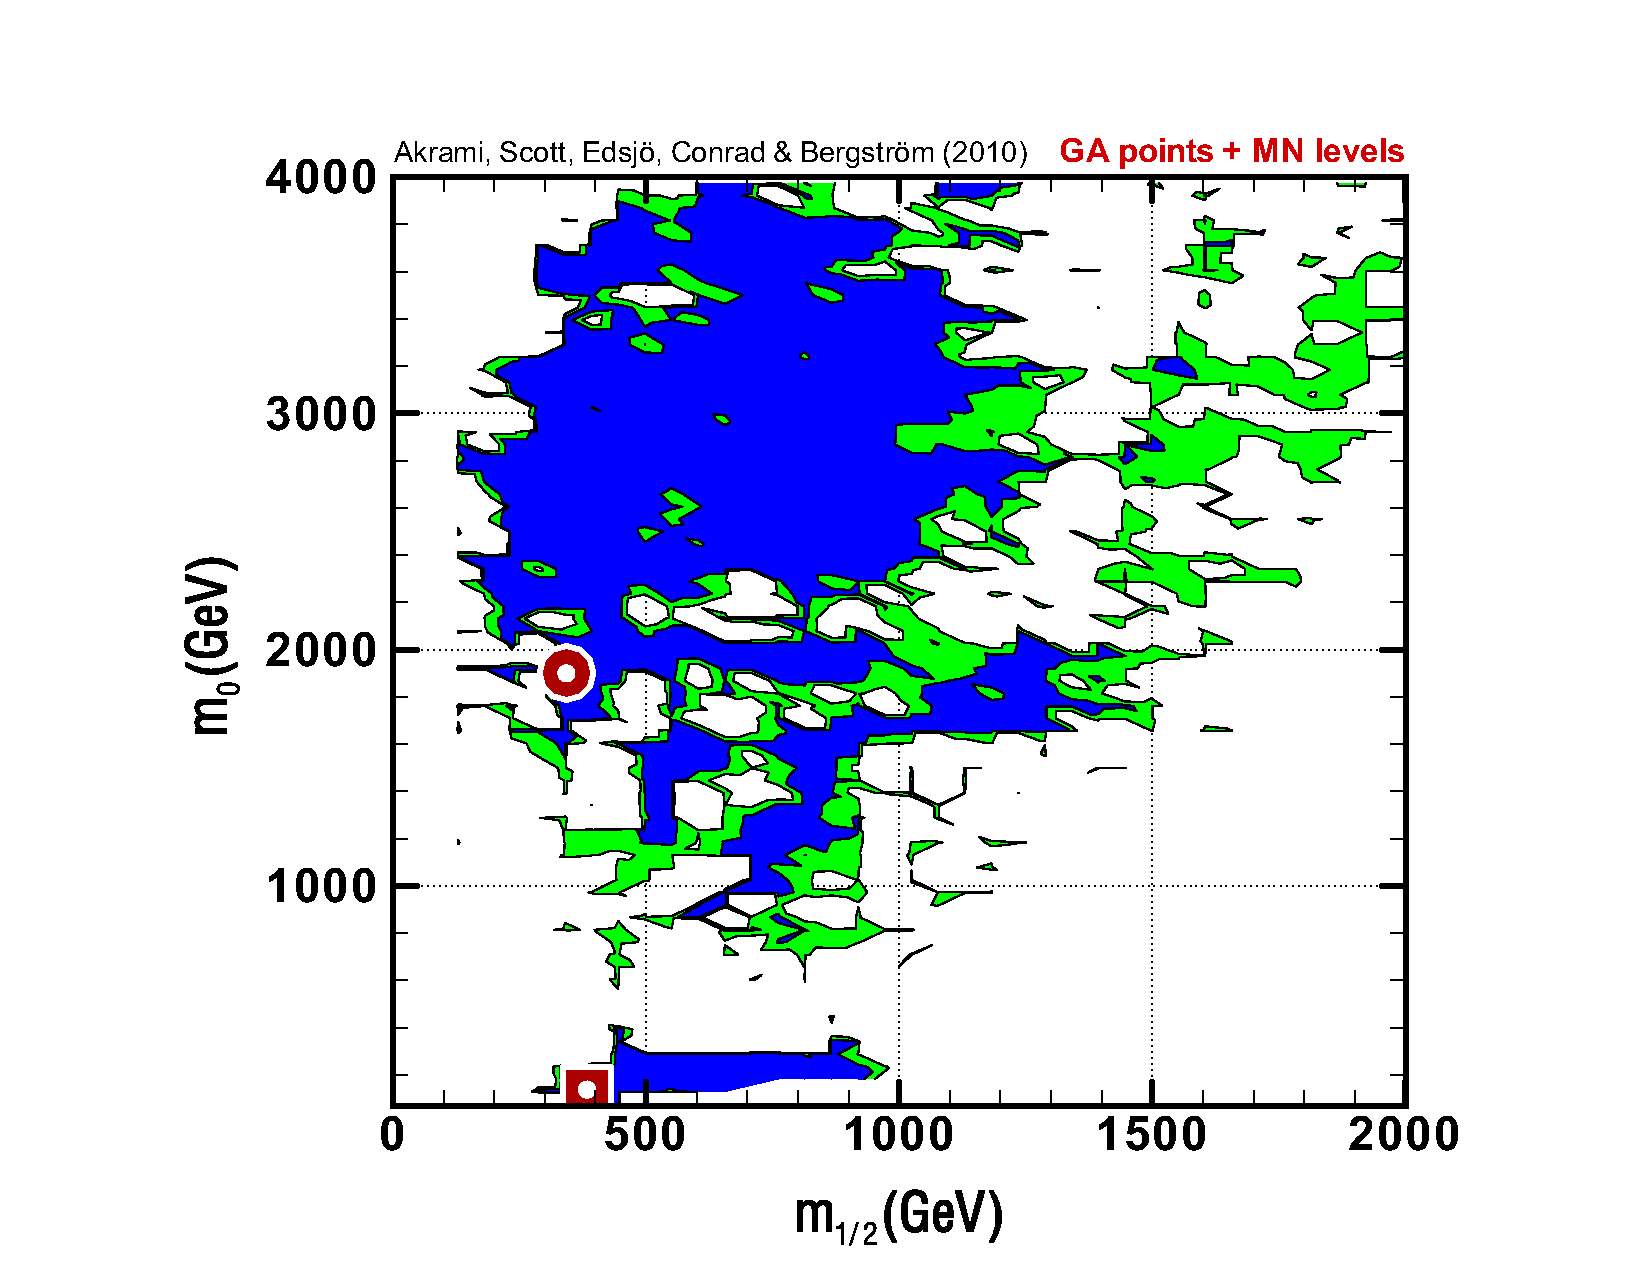
\includegraphics[width=0.5\textwidth]{GA_m0mhf_MNlevels}	


\end{frame}


\begin{frame}
\frametitle{Coverage [\alert{Statistical aside II}]}

{\scriptsize
\textbf{Test statistic}: a measure on data used to construct statistical tests (e.g. $\chi^2$, ln$\mathcal{L}$, etc.)\\
\textbf{Coverage}: the percentage of the time that a supposed `$x\%$' confidence region\\ actually contains the true value\\
\begin{itemize}
\item Distribution of the test statistic and design of the test it's used in determine coverage.
\item $p$-value calculation \textit{requires} the test statistic distribution to be well known.
\end{itemize}
}\vspace{3mm}

\cblue{We don't \textit{*really*} know the distribution of our test statistic in BSM global fits, as it is too expensive to Monte Carlo}
      \begin{itemize}\footnotesize
                 \item coverage is rarely spot-on unless mapping from parameters to data-space is linear \\
                 {\tiny(Akrami, Savage, PS et al {\it JCAP}, 1011.4297, Bridges et al {\it JHEP}, 1011.4306, Strege et al {\it PRD}, 1201.3631)}
                 \item $p$-value assessments of goodness of fit should be viewed with serious scepticism ($\rightarrow$MasterCode)
                 \end{itemize}

\end{frame}

\begin{frame}
\frametitle{Advanced IceCube Likelihood for Model Testing}

Simplest way to do anything is to first make it a counting problem\ldots

\vspace{3mm}

Compare observed number of events $n$ and predicted number $\theta$ for each model, taking into account error $\sigma_\epsilon$ on acceptance:

\begin{equation}
\label{fancy}
\scriptsize
\Like_\mathrm{num}(n|\theta_\mathrm{BG}+\theta_\mathrm{sig}) = \frac{1}{\sqrt{2\pi}\sigma_\epsilon}\int_0^\infty \frac{(\theta_\mathrm{BG}+\epsilon\theta_\mathrm{sig})^{n}e^{-(\theta_\mathrm{BG}+\epsilon\theta_\mathrm{sig})}}{n!}\frac1\epsilon\exp\left[-\frac{1}{2}\left(\frac{\ln\epsilon}{\sigma_\epsilon}\right)^2\right]\mathrm{d}\epsilon \, .
\end{equation}

\only<1>{Nuisance parameter $\epsilon$ takes into account systematic errors on effective area, etc.  $\sigma_\epsilon\sim20\%$ for IceCube.\vspace{2.17cm}}%
\only<2>{\alert{Then:} upgrade to full unbinned likelihood with number ($\Like_\mathrm{num}$), spectral ($\Like_\mathrm{spec}$) and angular ($\Like_\mathrm{ang}$) bits: 
\begin{equation}
\footnotesize
\Like = \Like_\mathrm{num}(n|\theta_{\mathrm{signal+BG}})\prod_{i=1}^{n} \Like_{\mathrm{spec},i}\,\Like_{\mathrm{ang},i}
\end{equation}

{\alert{All available in DarkSUSY v5.0.6 and later: }{\color[rgb]{0.1, 0.0, 0.6}\href{www.darksusy.org}{www.darksusy.org}}
\vspace{3mm}}}

\end{frame}

\begin{frame}
\frametitle{Prospects for detection in the MSSM-25}
86-string IceCube vs Gamma Rays

\begin{center}
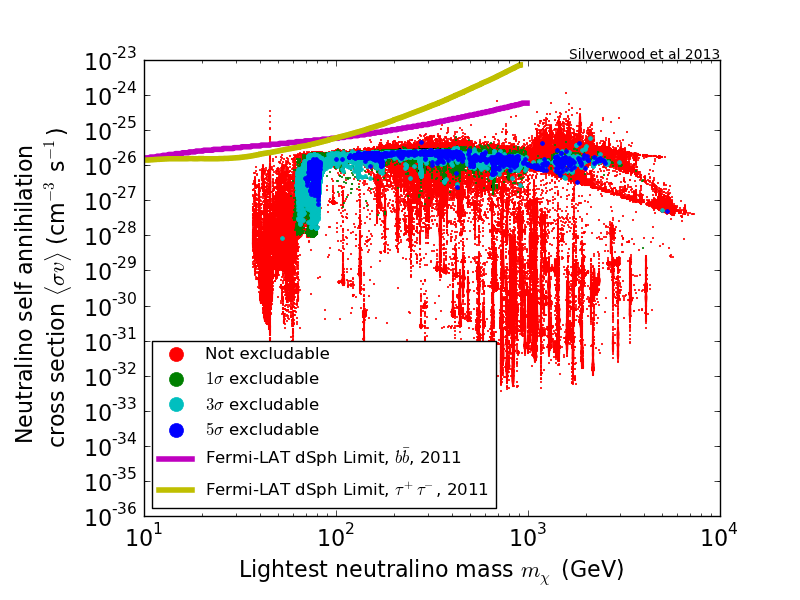
\includegraphics[width=0.65\textwidth]{MSSM25_ID}
\end{center}

Many models that IceCube-86 can see are not accessible by other indirect probes\ldots

\begin{textblock}{80}(75,72)
  {\tiny(Silverwood, PS, et al, \textit{JCAP}, 1210.0844)}
\end{textblock}

\end{frame}

\begin{frame}
\frametitle{Prospects for detection in the MSSM-25}
Gaugino fractions
\vspace{3mm}

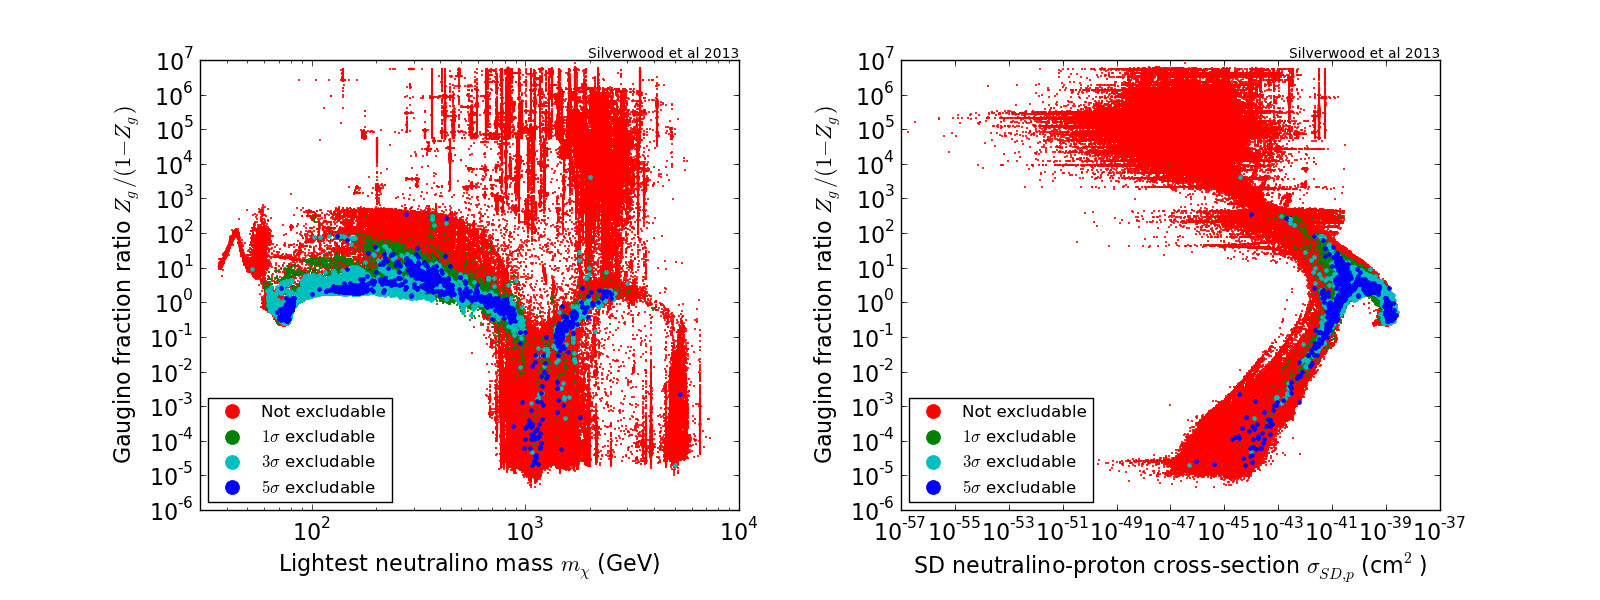
\includegraphics[width=1.1\textwidth, trim = 50 0 0 0, clip=true]{MSSM25_Gaugino}

\vspace{3mm}
Mainly mixed models, a few Higgsinos

\begin{textblock}{80}(75,72)
  {\tiny(Silverwood, PS, et al, \textit{JCAP}, 1210.0844)}
\end{textblock}

\end{frame}


\end{document}

